% ------------------------------------------------------------------------
% ------------------------------------------------------------------------
% Modelo UFSC para Trabalhos Academicos (tese de doutorado, dissertação de
% mestrado) utilizando a classe abntex2
%
% Autor: Alisson Lopes Furlani
% 	Modificações:
%	- 27/08/2019: Alisson L. Furlani, add pacote 'glossaries' para listas
% - 30/10/2019: Alisson L. Furlani, adjusted some spacing errors and changed math fonts
% - 17/01/2019: Alisson L. Furlani, updated certification page
% - 03/03/2020: Luiz F. P. Droubi, change file to be used as a template with R.
% ------------------------------------------------------------------------
% ------------------------------------------------------------------------

\documentclass[
	% -- opções da classe memoir --
	12pt,				% tamanho da fonte
	%openright,			% capítulos começam em pág ímpar (insere página vazia caso preciso)
	oneside,			% para impressão no anverso. Oposto a twoside
	a4paper,			% tamanho do papel.
	% -- opções da classe abntex2 --
	chapter=TITLE,		% títulos de capítulos convertidos em letras maiúsculas
	section=TITLE,		% títulos de seções convertidos em letras maiúsculas
	%subsection=TITLE,	% títulos de subseções convertidos em letras maiúsculas
	%subsubsection=TITLE,% títulos de subsubseções convertidos em letras maiúsculas
	% -- opções do pacote babel --
	english,			% idioma adicional para hifenização
	%french,				% idioma adicional para hifenização
	%spanish,			% idioma adicional para hifenização
	brazil				% o último idioma é o principal do documento
	]{abntex2}

\usepackage{setup/ufrnthesisA4-alf}

\addbibresource{bib/thesis.bib}
\addbibresource{bib/references.bib}
\addbibresource{bib/pkgs.bib}

\usepackage[table]{xcolor}
\let\newfloat\undefined
\usepackage{floatrow}
\floatsetup[table]{capposition=top}
\floatsetup[figure]{capposition=top}

\newcommand{\pkg}[1]{{\normalfont\fontseries{b}\selectfont #1}}
\let\proglang=\textsf
\let\code=\texttt

\usepackage{color}
\usepackage{fancyvrb}
\newcommand{\VerbBar}{|}
\newcommand{\VERB}{\Verb[commandchars=\\\{\}]}
\DefineVerbatimEnvironment{Highlighting}{Verbatim}{commandchars=\\\{\}}
% Add ',fontsize=\small' for more characters per line
\usepackage{framed}
\definecolor{shadecolor}{RGB}{248,248,248}
\newenvironment{Shaded}{\begin{snugshade}}{\end{snugshade}}
\newcommand{\AlertTok}[1]{\textcolor[rgb]{0.94,0.16,0.16}{#1}}
\newcommand{\AnnotationTok}[1]{\textcolor[rgb]{0.56,0.35,0.01}{\textbf{\textit{#1}}}}
\newcommand{\AttributeTok}[1]{\textcolor[rgb]{0.13,0.29,0.53}{#1}}
\newcommand{\BaseNTok}[1]{\textcolor[rgb]{0.00,0.00,0.81}{#1}}
\newcommand{\BuiltInTok}[1]{#1}
\newcommand{\CharTok}[1]{\textcolor[rgb]{0.31,0.60,0.02}{#1}}
\newcommand{\CommentTok}[1]{\textcolor[rgb]{0.56,0.35,0.01}{\textit{#1}}}
\newcommand{\CommentVarTok}[1]{\textcolor[rgb]{0.56,0.35,0.01}{\textbf{\textit{#1}}}}
\newcommand{\ConstantTok}[1]{\textcolor[rgb]{0.56,0.35,0.01}{#1}}
\newcommand{\ControlFlowTok}[1]{\textcolor[rgb]{0.13,0.29,0.53}{\textbf{#1}}}
\newcommand{\DataTypeTok}[1]{\textcolor[rgb]{0.13,0.29,0.53}{#1}}
\newcommand{\DecValTok}[1]{\textcolor[rgb]{0.00,0.00,0.81}{#1}}
\newcommand{\DocumentationTok}[1]{\textcolor[rgb]{0.56,0.35,0.01}{\textbf{\textit{#1}}}}
\newcommand{\ErrorTok}[1]{\textcolor[rgb]{0.64,0.00,0.00}{\textbf{#1}}}
\newcommand{\ExtensionTok}[1]{#1}
\newcommand{\FloatTok}[1]{\textcolor[rgb]{0.00,0.00,0.81}{#1}}
\newcommand{\FunctionTok}[1]{\textcolor[rgb]{0.13,0.29,0.53}{\textbf{#1}}}
\newcommand{\ImportTok}[1]{#1}
\newcommand{\InformationTok}[1]{\textcolor[rgb]{0.56,0.35,0.01}{\textbf{\textit{#1}}}}
\newcommand{\KeywordTok}[1]{\textcolor[rgb]{0.13,0.29,0.53}{\textbf{#1}}}
\newcommand{\NormalTok}[1]{#1}
\newcommand{\OperatorTok}[1]{\textcolor[rgb]{0.81,0.36,0.00}{\textbf{#1}}}
\newcommand{\OtherTok}[1]{\textcolor[rgb]{0.56,0.35,0.01}{#1}}
\newcommand{\PreprocessorTok}[1]{\textcolor[rgb]{0.56,0.35,0.01}{\textit{#1}}}
\newcommand{\RegionMarkerTok}[1]{#1}
\newcommand{\SpecialCharTok}[1]{\textcolor[rgb]{0.81,0.36,0.00}{\textbf{#1}}}
\newcommand{\SpecialStringTok}[1]{\textcolor[rgb]{0.31,0.60,0.02}{#1}}
\newcommand{\StringTok}[1]{\textcolor[rgb]{0.31,0.60,0.02}{#1}}
\newcommand{\VariableTok}[1]{\textcolor[rgb]{0.00,0.00,0.00}{#1}}
\newcommand{\VerbatimStringTok}[1]{\textcolor[rgb]{0.31,0.60,0.02}{#1}}
\newcommand{\WarningTok}[1]{\textcolor[rgb]{0.56,0.35,0.01}{\textbf{\textit{#1}}}}

\newcommand{\bcenter}{\begin{center}}
\newcommand{\ecenter}{\end{center}}

\newcommand{\bapendices}{\begin{apendicesenv}}
\newcommand{\eapendices}{\end{apendicesenv}}

\newcommand{\banexos}{\begin{anexosenv}}
\newcommand{\eanexos}{\end{anexosenv}}

% ---
% Filtering and Mapping Bibliographies
% ---
\DeclareSourcemap{
	\maps[datatype=bibtex]{
		% remove fields that are always useless
		\map{
			\step[fieldset=abstract, null]
			\step[fieldset=pagetotal, null]
		}
		% remove URLs for types that are primarily printed
%		\map{
%			\pernottype{software}
%			\pernottype{online}
%			\pernottype{report}
%			\pernottype{techreport}
%			\pernottype{standard}
%			\pernottype{manual}
%			\pernottype{misc}
%			\step[fieldset=url, null]
%			\step[fieldset=urldate, null]
%		}
		\map{
			\pertype{inproceedings}
			% remove mostly redundant conference information
			\step[fieldset=venue, null]
			\step[fieldset=eventdate, null]
			\step[fieldset=eventtitle, null]
			% do not show ISBN for proceedings
			\step[fieldset=isbn, null]
			% Citavi bug
			\step[fieldset=volume, null]
		}
	}
}
% ---

% ---
% Informações de dados para CAPA e FOLHA DE ROSTO
% ---
% FIXME Substituir 'Nome completo do autor' pelo seu nome.
\autor{JOÃO VITOR FERREIRA CAVALCANTE}
% FIXME Substituir 'Título do trabalho' pelo título da trabalho.
\titulo{TÍTULO DE METAGENÔMICA}
% FIXME Substituir 'Subtítulo (se houver)' pelo subtítulo da trabalho.
% Caso não tenha substítulo, comente a linha a seguir.
  \subtitulo{SUBTÍTULO}
% FIXME Substituir 'XXXXXX' pelo nome do seu
% orientador.
\orientador{Rodrigo Juliani Siqueira Dalmolin}
% FIXME Se for orientado por uma mulher, comente a linha acima e descomente a linha a seguir.
% \orientador[Orientadora]{Nome da orientadora, Dra.}
% FIXME Substituir 'XXXXXX' pelo nome do seu
% coorientador. Caso não tenha coorientador, comente a linha a seguir.
% FIXME Se for coorientado por uma mulher, comente a linha acima e descomente a linha a seguir.
% \coorientador[Coorientadora]{XXXXXX, Dra.}
% FIXME Substituir '[ano]' pelo ano (ano) em que seu trabalho foi defendido.
\ano{2024}
% FIXME Substituir '[dia] de [mês] de [ano]' pela data em que ocorreu sua defesa.
\data{31 de Setembro de 2024}
% FIXME Substituir 'Local' pela cidade em que ocorreu sua defesa.
\local{NATAL - RN}
\instituicaosigla{UFRN}
\instituicao{Universidade Federal do Rio Grande do Norte}
% FIXME Substituir 'Dissertação/Tese' pelo tipo de trabalho (Tese, Dissertação).
\tipotrabalho{Defesa de Mestrado}
% FIXME Substituir '[mestre/doutor] em XXXXXX' pela grau adequado.
\formacao{Mestre em Bioinformática}
% FIXME Substituir '[mestrado/doutorado]' pelo nivel adequado.
\nivel{mestrado}
% FIXME Substituir 'Programa de Pós-Graduação em XXXXXX' pela curso adequado.
\programa{Programa de Pós-Graduação em Bioinformática}
% FIXME Substituir 'Campus XXXXXX ou Centro de XXXXXX' pelo campus ou centro adequado.
\centro{Instituto Metrópole Digital}
\preambulo
{%
\imprimirtipotrabalho~apresentada~ao~\imprimirprograma~da~\imprimirinstituicao.
}
% ---

% ---
% Configurações de aparência do PDF final
% ---
% alterando o aspecto da cor azul
\definecolor{blue}{RGB}{41,5,195}
% informações do PDF
\makeatletter
\hypersetup{
     	%pagebackref=true,
		pdftitle={\@title},
		pdfauthor={\@author},
    	pdfsubject={\imprimirpreambulo},
	    pdfcreator={LaTeX with abnTeX2},
		pdfkeywords={ufsc, latex, abntex2},
		colorlinks=true,       		% false: boxed links; true: colored links
    	linkcolor=black,%blue,          	% color of internal links
    	citecolor=black,%blue,        		% color of links to bibliography
    	filecolor=black,%magenta,      		% color of file links
		urlcolor=black,%blue,
		bookmarksdepth=4
}
\makeatother
% ---

% ---
% compila a lista de abreviaturas e siglas e a lista de símbolos
% ---

% Declaração das siglas
\siglalista{MS}{metagenômica \textit{shotgun}}
\siglalista{16S}{sequenciamento da subunidade ribossomal 16S de genomas bacterianos}
\siglalista{TDM}{transtorno depressivo maior}
\siglalista{DNA}{Ácido Desoxirribonucléico}
\siglalista{OTU}{unidades taxonômicas operacionais - do inglês \textit{operational taxonomic units}}
\siglalista{ASV}{variantes de sequência amplicon - do inglês \textit{amplicon sequence variant}}


% Declaração dos simbolos
\simbololista{C}{\ensuremath{C}}{Circunferência de um círculo}
\simbololista{pi}{\ensuremath{\pi}}{Número pi}
\simbololista{r}{\ensuremath{r}}{Raio de um círculo}
\simbololista{A}{\ensuremath{A}}{Área de um círculo}


% compila a lista de abreviaturas e siglas e a lista de símbolos
\makenoidxglossaries

% ---

% ---
% compila o indice
% ---
\makeindex
% ---

% ----
% Início do documento
% ----
\begin{document}

% Seleciona o idioma do documento (conforme pacotes do babel)
%\selectlanguage{english}
\selectlanguage{brazil}

% Retira espaço extra obsoleto entre as frases.
\frenchspacing

% Espaçamento 1.5 entre linhas
\OnehalfSpacing

% Corrige justificação
%\sloppy

% ----------------------------------------------------------
% ELEMENTOS PRÉ-TEXTUAIS
% ----------------------------------------------------------
% \pretextual %a macro \pretextual é acionado automaticamente no início de \begin{document}
% ---
% Capa, folha de rosto, ficha bibliografica, errata, folha de apróvação
% Dedicatória, agradecimentos, epígrafe, resumos, listas
% ---
% ---
% Capa
% ---
\imprimircapa
% ---

% ---
% Folha de rosto
% (o * indica que haverá a ficha bibliográfica)
% ---
\imprimirfolhaderosto*
% ---

% ---
% Inserir a ficha bibliografica
% ---
% http://ficha.bu.ufsc.br/
% \begin{fichacatalografica}
% 	\includepdf{Ficha_Catalografica.pdf}
% \end{fichacatalografica}
% ---

% ---
% Inserir folha de aprovação
% ---
\begin{folhadeaprovacao}
	\OnehalfSpacing
	% \centering
	\begin{center}
	\imprimirautor\\%
	\vspace*{10pt}
	\textbf{\imprimirtitulo}%
	\ifnotempty{\imprimirsubtitulo}{:~\imprimirsubtitulo}\\%
	%		\vspace*{31.5pt}%3\baselineskip
	\vspace*{\baselineskip}
	\end{center}
	%\begin{minipage}{\textwidth}
	\imprimirtipotrabalho~apresentada~ao~\imprimirprograma~da~\imprimirinstituicao\\
	%\end{minipage}%
	\bigskip\newline
	\textbf{Área de Concentração}:~Bioinformática\newline%
	\textbf{Linha de Pesquisa}:~Biologia de Sistemas\newline%
	\imprimirorientadorRotulo:~\imprimirorientador\newline%
	\begin{flushright}
	Natal, \imprimirdata.
	\end{flushright}
	\vspace*{\baselineskip}
  %   % Prof. Examinador 1, Dr.\\
  % Universidade Federal do Rio Grande do Norte - UFRN\\
  % \vspace*{\baselineskip}
  %   % Prof. Examinador 2, Dr.\\
  % Universidade Federal dos Externos - UFE\\
  % \vspace*{\baselineskip}
  % 
	\vspace*{2\baselineskip}
	% \begin{minipage}{\textwidth}
	% 	Certificamos que esta é a \textbf{versão original e final} do trabalho de conclusão que foi julgado adequado para obtenção do título de \imprimirformacao.\\
	% \end{minipage}
	%    \vspace{-0.7cm}
	\centering{\textbf{BANCA EXAMINADORA}}
	\assinatura{\OnehalfSpacing Prof. Dr. \imprimirorientador \\ \footnotesize{\imprimirinstituicao \\ (Presidente)}}
    \assinatura{Prof. Dr. Examinador 1 \\ \footnotesize{Universidade Federal do Rio Grande do Norte \\ (Examinador Interno do Programa)}}
    \assinatura{Prof. Dr. Examinador 2 \\ \footnotesize{Universidade Federal dos Externos \\ (Examinador Externo à Instituição)}}
  	%	\ifnotempty{\imprimircoorientador}{
	%	\assinatura{\imprimircoorientador \\ \imprimircoorientadorRotulo \\
	%		\imprimirinstituicao~--~\imprimirinstituicaosigla}
	%	}
	% \newpage
	\vspace*{\fill}
	\centering
\end{folhadeaprovacao}
% ---

% ---
% Dedicatória
% ---
% \begin{dedicatoria}
% 	\vspace*{\fill}
% 	\noindent
% 	\begin{adjustwidth*}{}{5.5cm}
% 		\raggedleft
% 		Este trabalho é dedicado a algumas pessoas.
% 	\end{adjustwidth*}
% \end{dedicatoria}
% ---

% ---
% Agradecimentos
% ---
\begin{agradecimentos}
	Gostaria de agradecer sinceramente a todos os que colaboraram à execução\\
deste trabalho.
\end{agradecimentos}
% ---

% ---
% Epígrafe
% ---
\begin{epigrafe}
	\vspace*{\fill}
	\begin{flushright}
		\textit{``Eppur si muove!''\\
(Galileu Galilei, 1633)}
	\end{flushright}
\end{epigrafe}
% ---

% ---
% RESUMOS
% ---

% resumo em português
\setlength{\absparsep}{18pt} % ajusta o espaçamento dos parágrafos do resumo
\begin{resumo}
	\SingleSpacing
  No resumo são ressaltados o objetivo da pesquisa, o método utilizado, as discussões e os resultados com destaque apenas para os pontos principais. O resumo deve ser significativo, composto de uma sequência de frases concisas, afirmativas, e não de uma enumeração de tópicos. Não deve conter citações. Deve usar o verbo na voz ativa e na terceira pessoa do singular. O texto do resumo deve ser digitado, em um único bloco, sem espaço de parágrafo. O espaçamento entre linhas é simples e o tamanho da fonte é 12. Abaixo do resumo, informar as palavras-chave (palavras ou expressões significativas retiradas do texto) ou, termos retirados de thesaurus da área. Deve conter de 150 a 500 palavras. O resumo é elaborado de acordo com a NBR 6028.

  \textbf{Palavras-chave}:
    Palavra-chave 1.
    Palavra-chave 2.
  \end{resumo}
% resumo em inglês
\begin{resumo}[Abstract]
	\SingleSpacing
	\begin{otherlanguage*}{english}
		Resumo traduzido para outros idiomas, neste caso, inglês. Segue o formato do resumo feito na língua vernácula. As palavras-chave traduzidas, versão em língua estrangeira, são colocadas abaixo do texto precedidas pela expressão ``Keywords'', separadas por ponto.

		\textbf{Keywords}:
	      Keyword 1.
        Keyword 2.
    	\end{otherlanguage*}
\end{resumo}
%% resumo em francês
%\begin{resumo}[Résumé]
% \begin{otherlanguage*}{french}
%    Il s'agit d'un résumé en français.
%
%   \textbf{Mots-clés}: latex. abntex. publication de textes.
% \end{otherlanguage*}
%\end{resumo}
%
%% resumo em espanhol
%\begin{resumo}[Resumen]
% \begin{otherlanguage*}{spanish}
%   Este es el resumen en español.
%
%   \textbf{Palabras clave}: latex. abntex. publicación de textos.
% \end{otherlanguage*}
%\end{resumo}
%% ---

{%hidelinks
	\hypersetup{hidelinks}
	% ---
	% inserir lista de ilustrações
	% ---
	\pdfbookmark[0]{\listfigurename}{lof}
	\listoffigures*
	\cleardoublepage
	% ---

	% ---
	% inserir lista de quadros
	% ---
	\pdfbookmark[0]{\listofquadrosname}{loq}
	\listofquadros*
	\cleardoublepage
	% ---

	% ---
	% inserir lista de tabelas
	% ---
	\pdfbookmark[0]{\listtablename}{lot}
	\listoftables*
	\cleardoublepage
	% ---

	% ---
	% inserir lista de abreviaturas e siglas (devem ser declarados no preambulo)
	% ---
	\imprimirlistadesiglas
	% ---

	% ---
	% inserir lista de símbolos (devem ser declarados no preambulo)
	% ---
	\imprimirlistadesimbolos
	% ---

	% ---
	% inserir o sumario
	% ---
	\pdfbookmark[0]{\contentsname}{toc}
	\tableofcontents*
	\cleardoublepage

}%hidelinks
% ---

% ---

% ----------------------------------------------------------
% ELEMENTOS TEXTUAIS
% ----------------------------------------------------------
\textual

\chapter{Introdução}\label{intro}

As orientações aqui apresentadas são baseadas em um conjunto de normas
elaboradas pela \gls{ABNT}. Além das normas técnicas, a Biblioteca também
elaborou uma série de tutoriais, guias, \emph{templates} os quais estão disponíveis
em seu site, no endereço \url{http://portal.bu.ufsc.br/normalizacao/}.

Paralelamente ao uso deste \emph{template} recomenda-se que seja utilizado o
\textbf{Tutorial de Trabalhos Acadêmicos} (disponível neste
\href{/url\%7Bhttps://repositorio.ufsc.br/handle/123456789/180829}{link}) e/ou que o
discente \textbf{participe das capacitações oferecidas da Biblioteca Universitária da
UFSC}.

Este \emph{template} está configurado apenas para a impressão utilizando o
anverso das folhas, caso você queira imprimir usando a frente e o verso,
acrescente a opção \emph{openright} e mude de \emph{oneside} para
\emph{twoside} nas configurações da classe \emph{abntex2} no início do
arquivo principal \emph{main.tex} \autocite{abntex2classe}.

Conforme a \href{https://repositorio.ufsc.br/bitstream/handle/123456789/197121/RN46.2019.pdf?sequence=1&isAllowed=y}{Resolução NORMATIVA nº 46/2019/CPG}
as dissertações e teses não serão mais entregues em formato impresso na
Biblioteca Universitária. Consulte o Repositório Institucional da UFSC ou sua
Secretaria de Pós Graduação sobre os procedimentos para a entrega.

\chapter{Objetivos}\label{objetivos}

Nas seções abaixo estão descritos o objetivo geral e os objetivos
específicos.

\section{Geral}\label{geral}

Descrição\ldots{}\gls{Bacen}

\section{Específicos}\label{especuxedficos}

Descrição\ldots{}

\chapter*{Capítulo 1}\label{cap1}
\addcontentsline{toc}{chapter}{Capítulo 1}

Deve-se inserir texto entre as seções.

\chapter*{Capítulo 2}\label{cap2}
\addcontentsline{toc}{chapter}{Capítulo 2}

Este \emph{template} contém algumas seções criadas na tentativa de facilitar seu uso.
No entanto, não há um limite máximo ou mínimo de seção a ser utilizado no
trabalho. Cabe a cada autor definir a quantidade que melhor atenda à sua
necessidade.

Para criar figuras com o \proglang{R}, pode-se seguir o padrão do código
abaixo, utilizado para produzir as imagens da figura \ref{fig:anscombe}:
\begin{Shaded}
\begin{Highlighting}[]
\FunctionTok{data}\NormalTok{(anscombe)}
\FunctionTok{plot}\NormalTok{(y1}\SpecialCharTok{\textasciitilde{}}\NormalTok{x1, }\AttributeTok{data =}\NormalTok{ anscombe)}
\FunctionTok{abline}\NormalTok{(}\FunctionTok{lm}\NormalTok{(y1}\SpecialCharTok{\textasciitilde{}}\NormalTok{x1, }\AttributeTok{data =}\NormalTok{ anscombe))}
\FunctionTok{plot}\NormalTok{(y2}\SpecialCharTok{\textasciitilde{}}\NormalTok{x2, }\AttributeTok{data =}\NormalTok{ anscombe)}
\FunctionTok{abline}\NormalTok{(}\FunctionTok{lm}\NormalTok{(y2}\SpecialCharTok{\textasciitilde{}}\NormalTok{x2, }\AttributeTok{data =}\NormalTok{ anscombe))}
\FunctionTok{plot}\NormalTok{(y3}\SpecialCharTok{\textasciitilde{}}\NormalTok{x3, }\AttributeTok{data =}\NormalTok{ anscombe)}
\FunctionTok{abline}\NormalTok{(}\FunctionTok{lm}\NormalTok{(y3}\SpecialCharTok{\textasciitilde{}}\NormalTok{x3, }\AttributeTok{data =}\NormalTok{ anscombe))}
\FunctionTok{plot}\NormalTok{(y4}\SpecialCharTok{\textasciitilde{}}\NormalTok{x4, }\AttributeTok{data =}\NormalTok{ anscombe)}
\FunctionTok{abline}\NormalTok{(}\FunctionTok{lm}\NormalTok{(y4}\SpecialCharTok{\textasciitilde{}}\NormalTok{x4, }\AttributeTok{data =}\NormalTok{ anscombe))}
\end{Highlighting}
\end{Shaded}
\begin{figure}[H]

{\centering 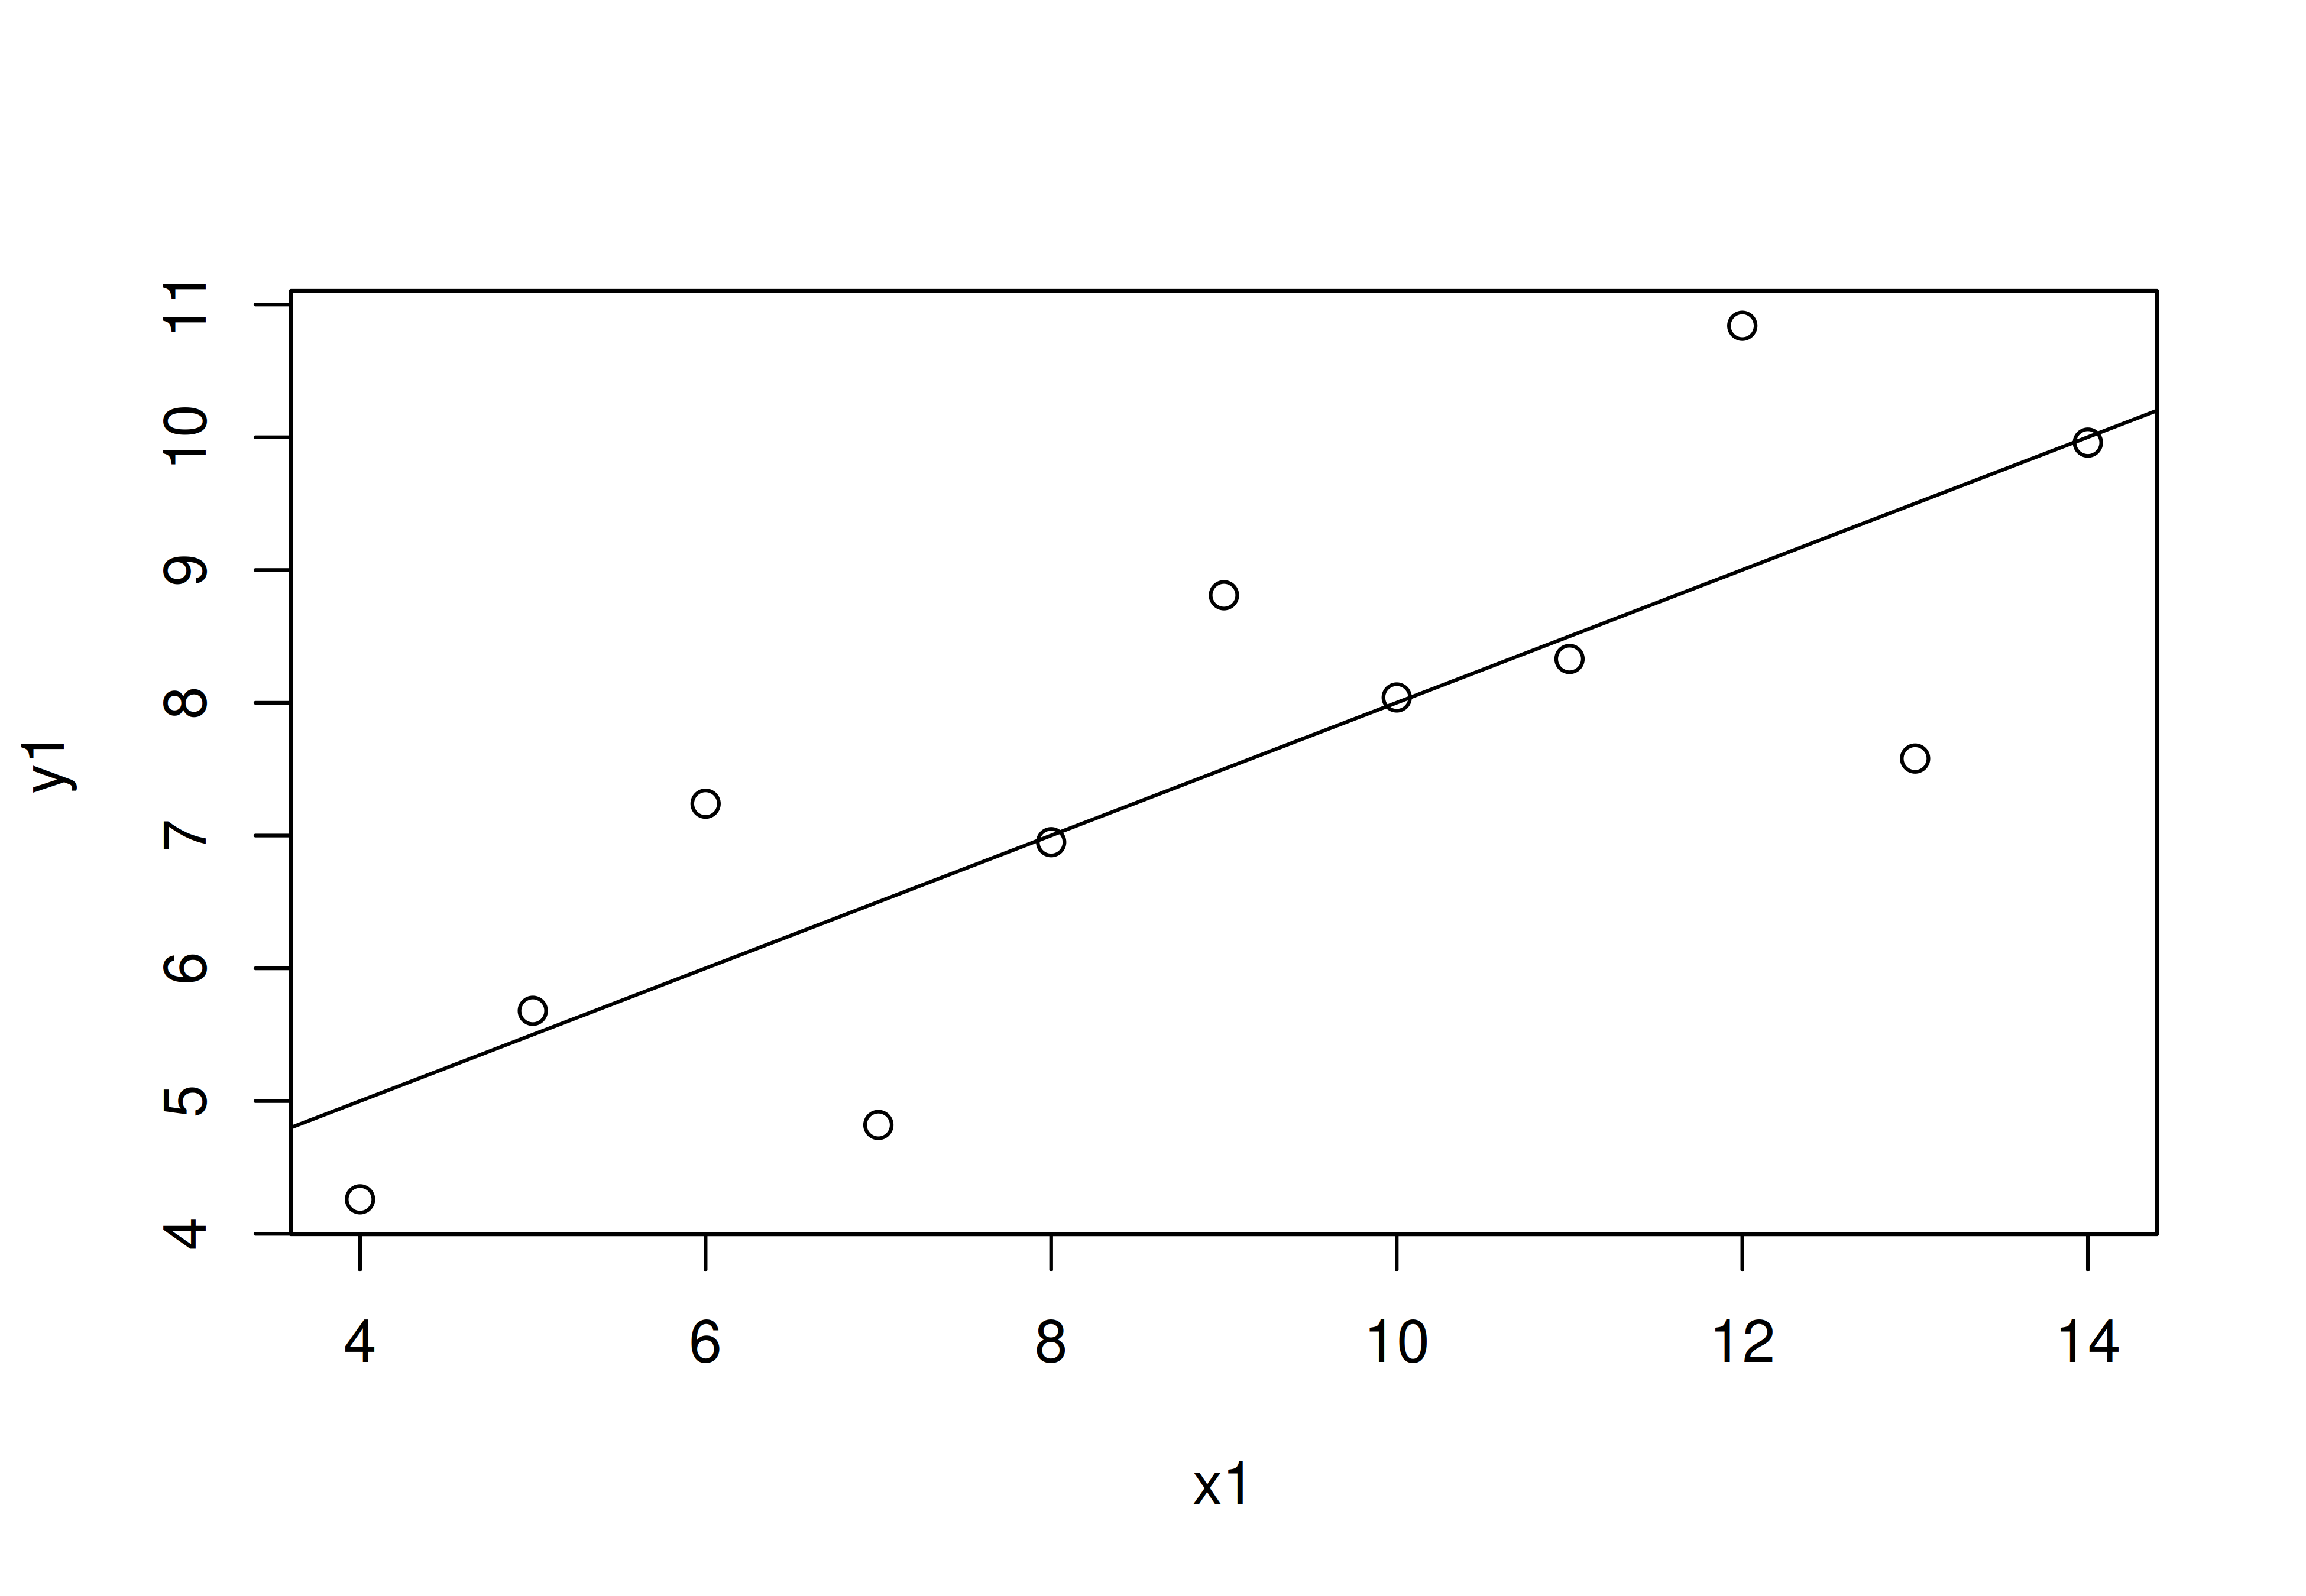
\includegraphics[width=0.49\linewidth]{images/anscombe-1} 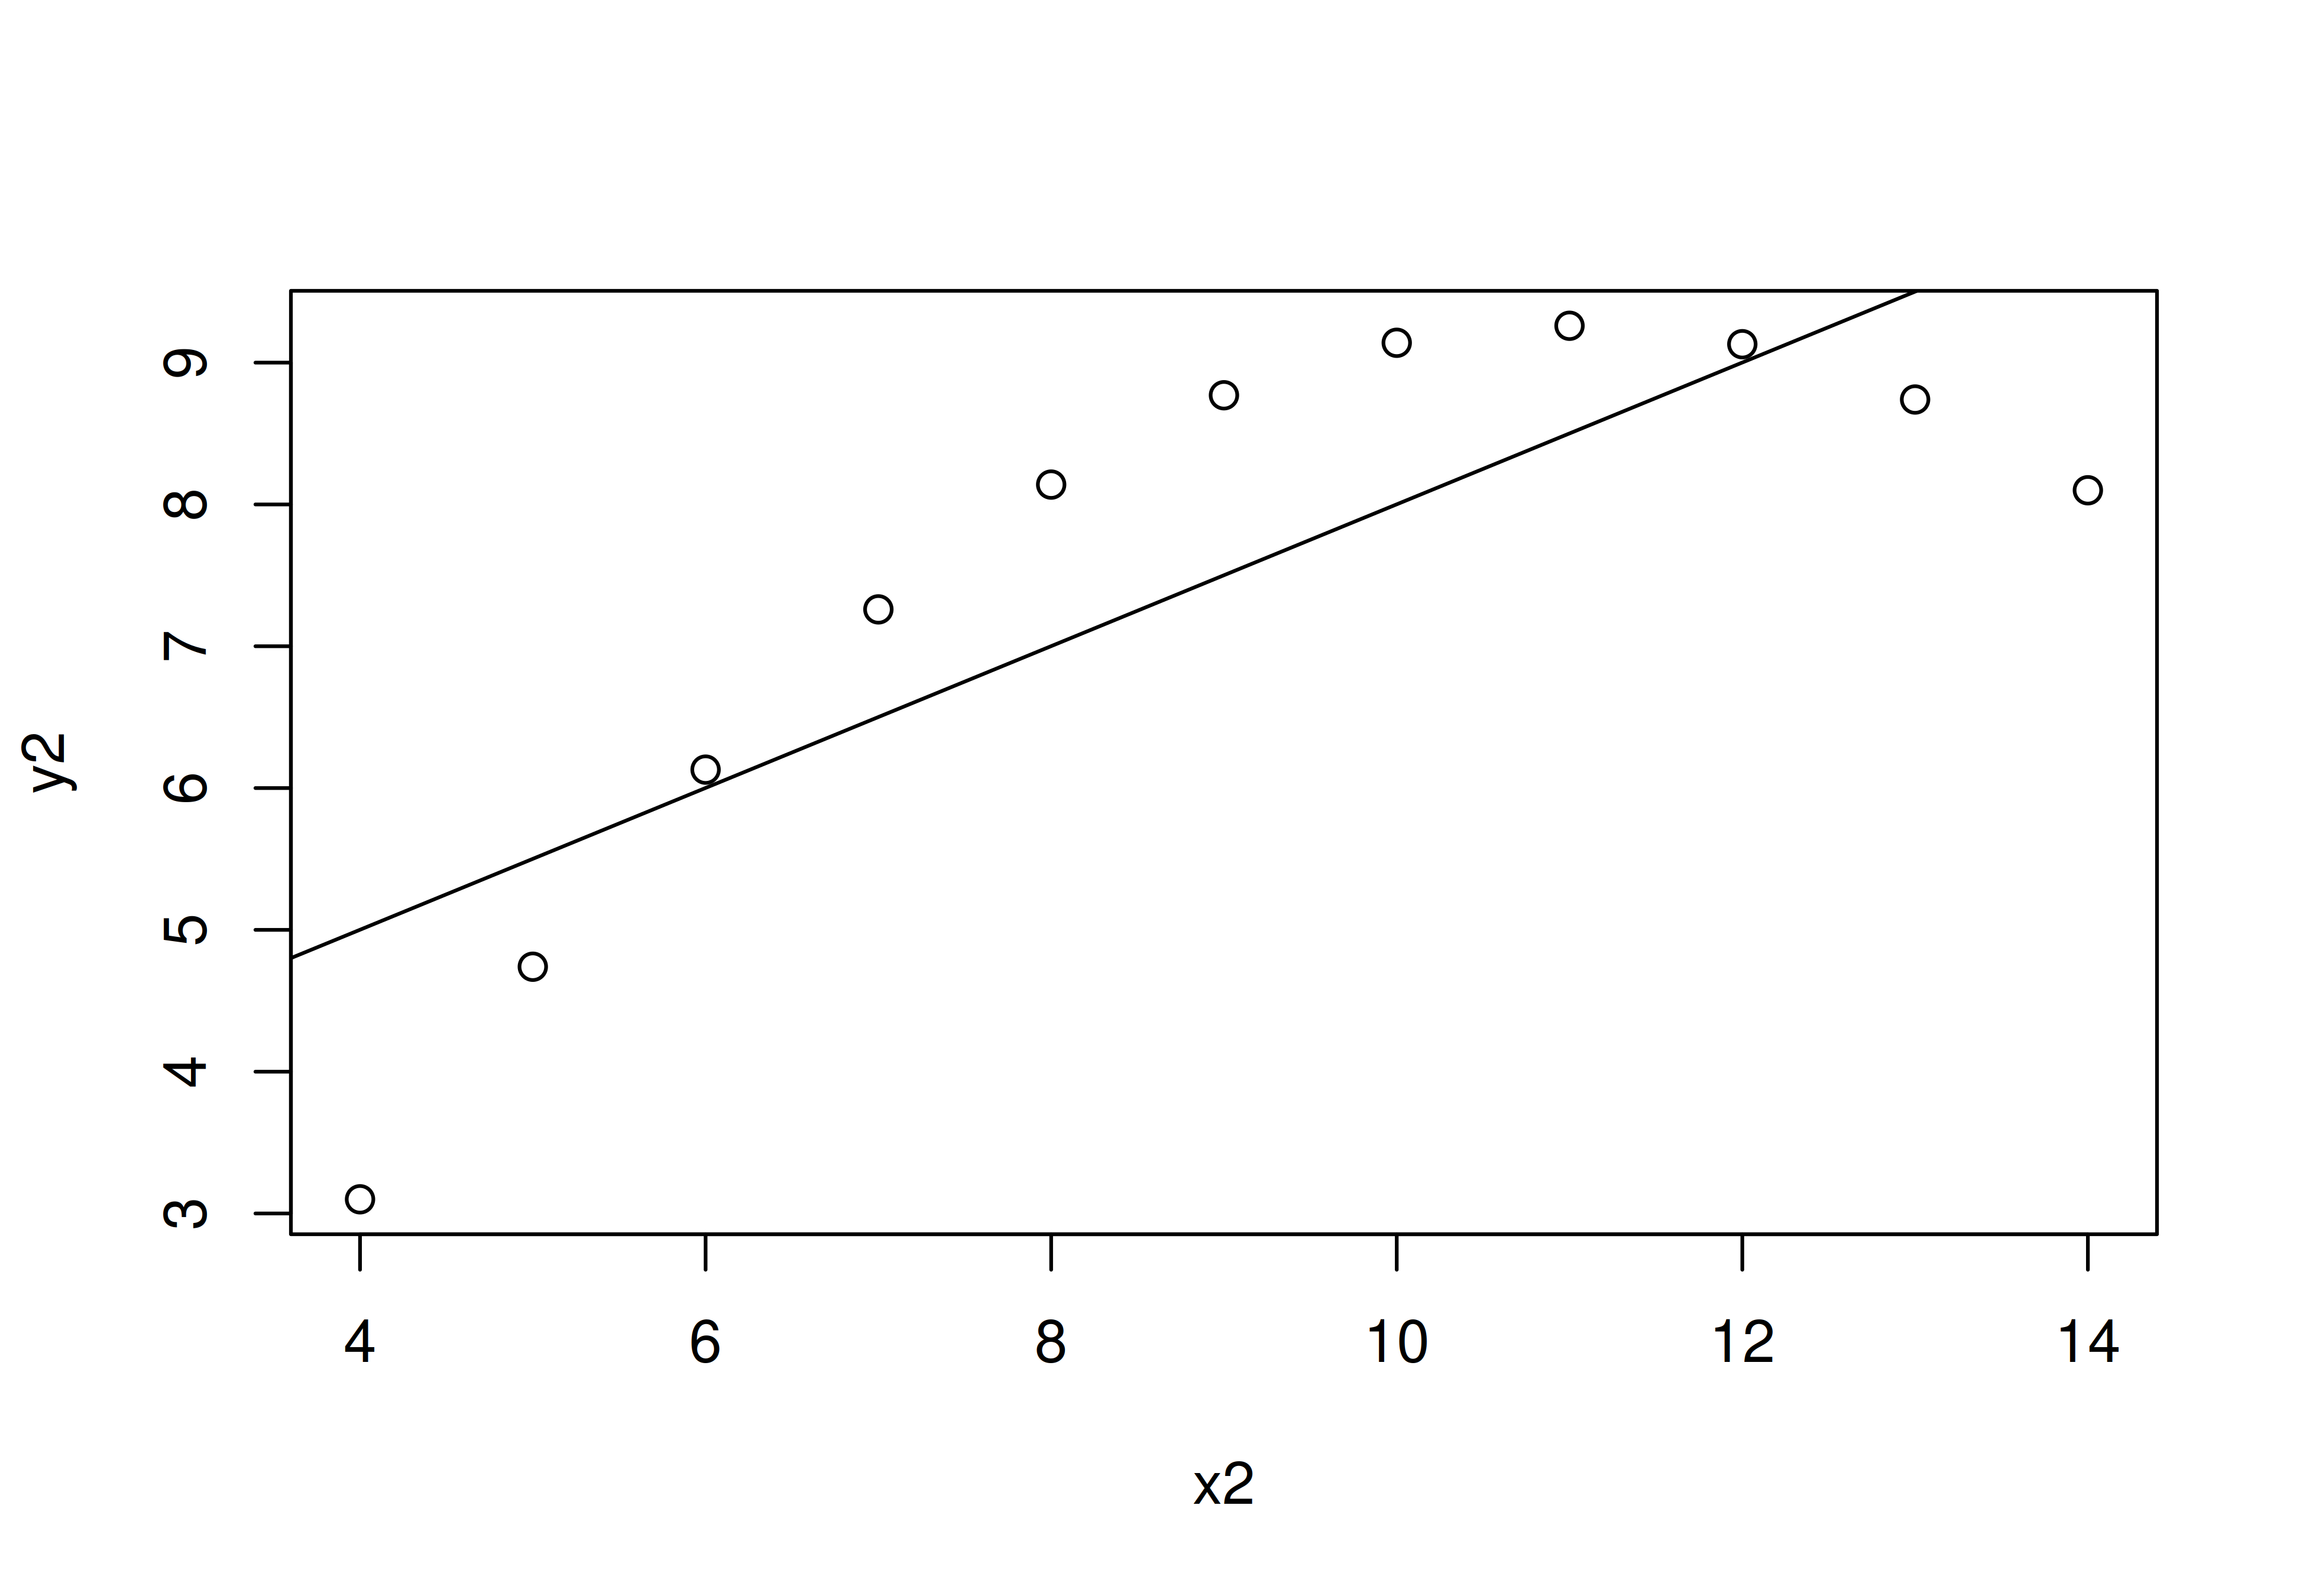
\includegraphics[width=0.49\linewidth]{images/anscombe-2} 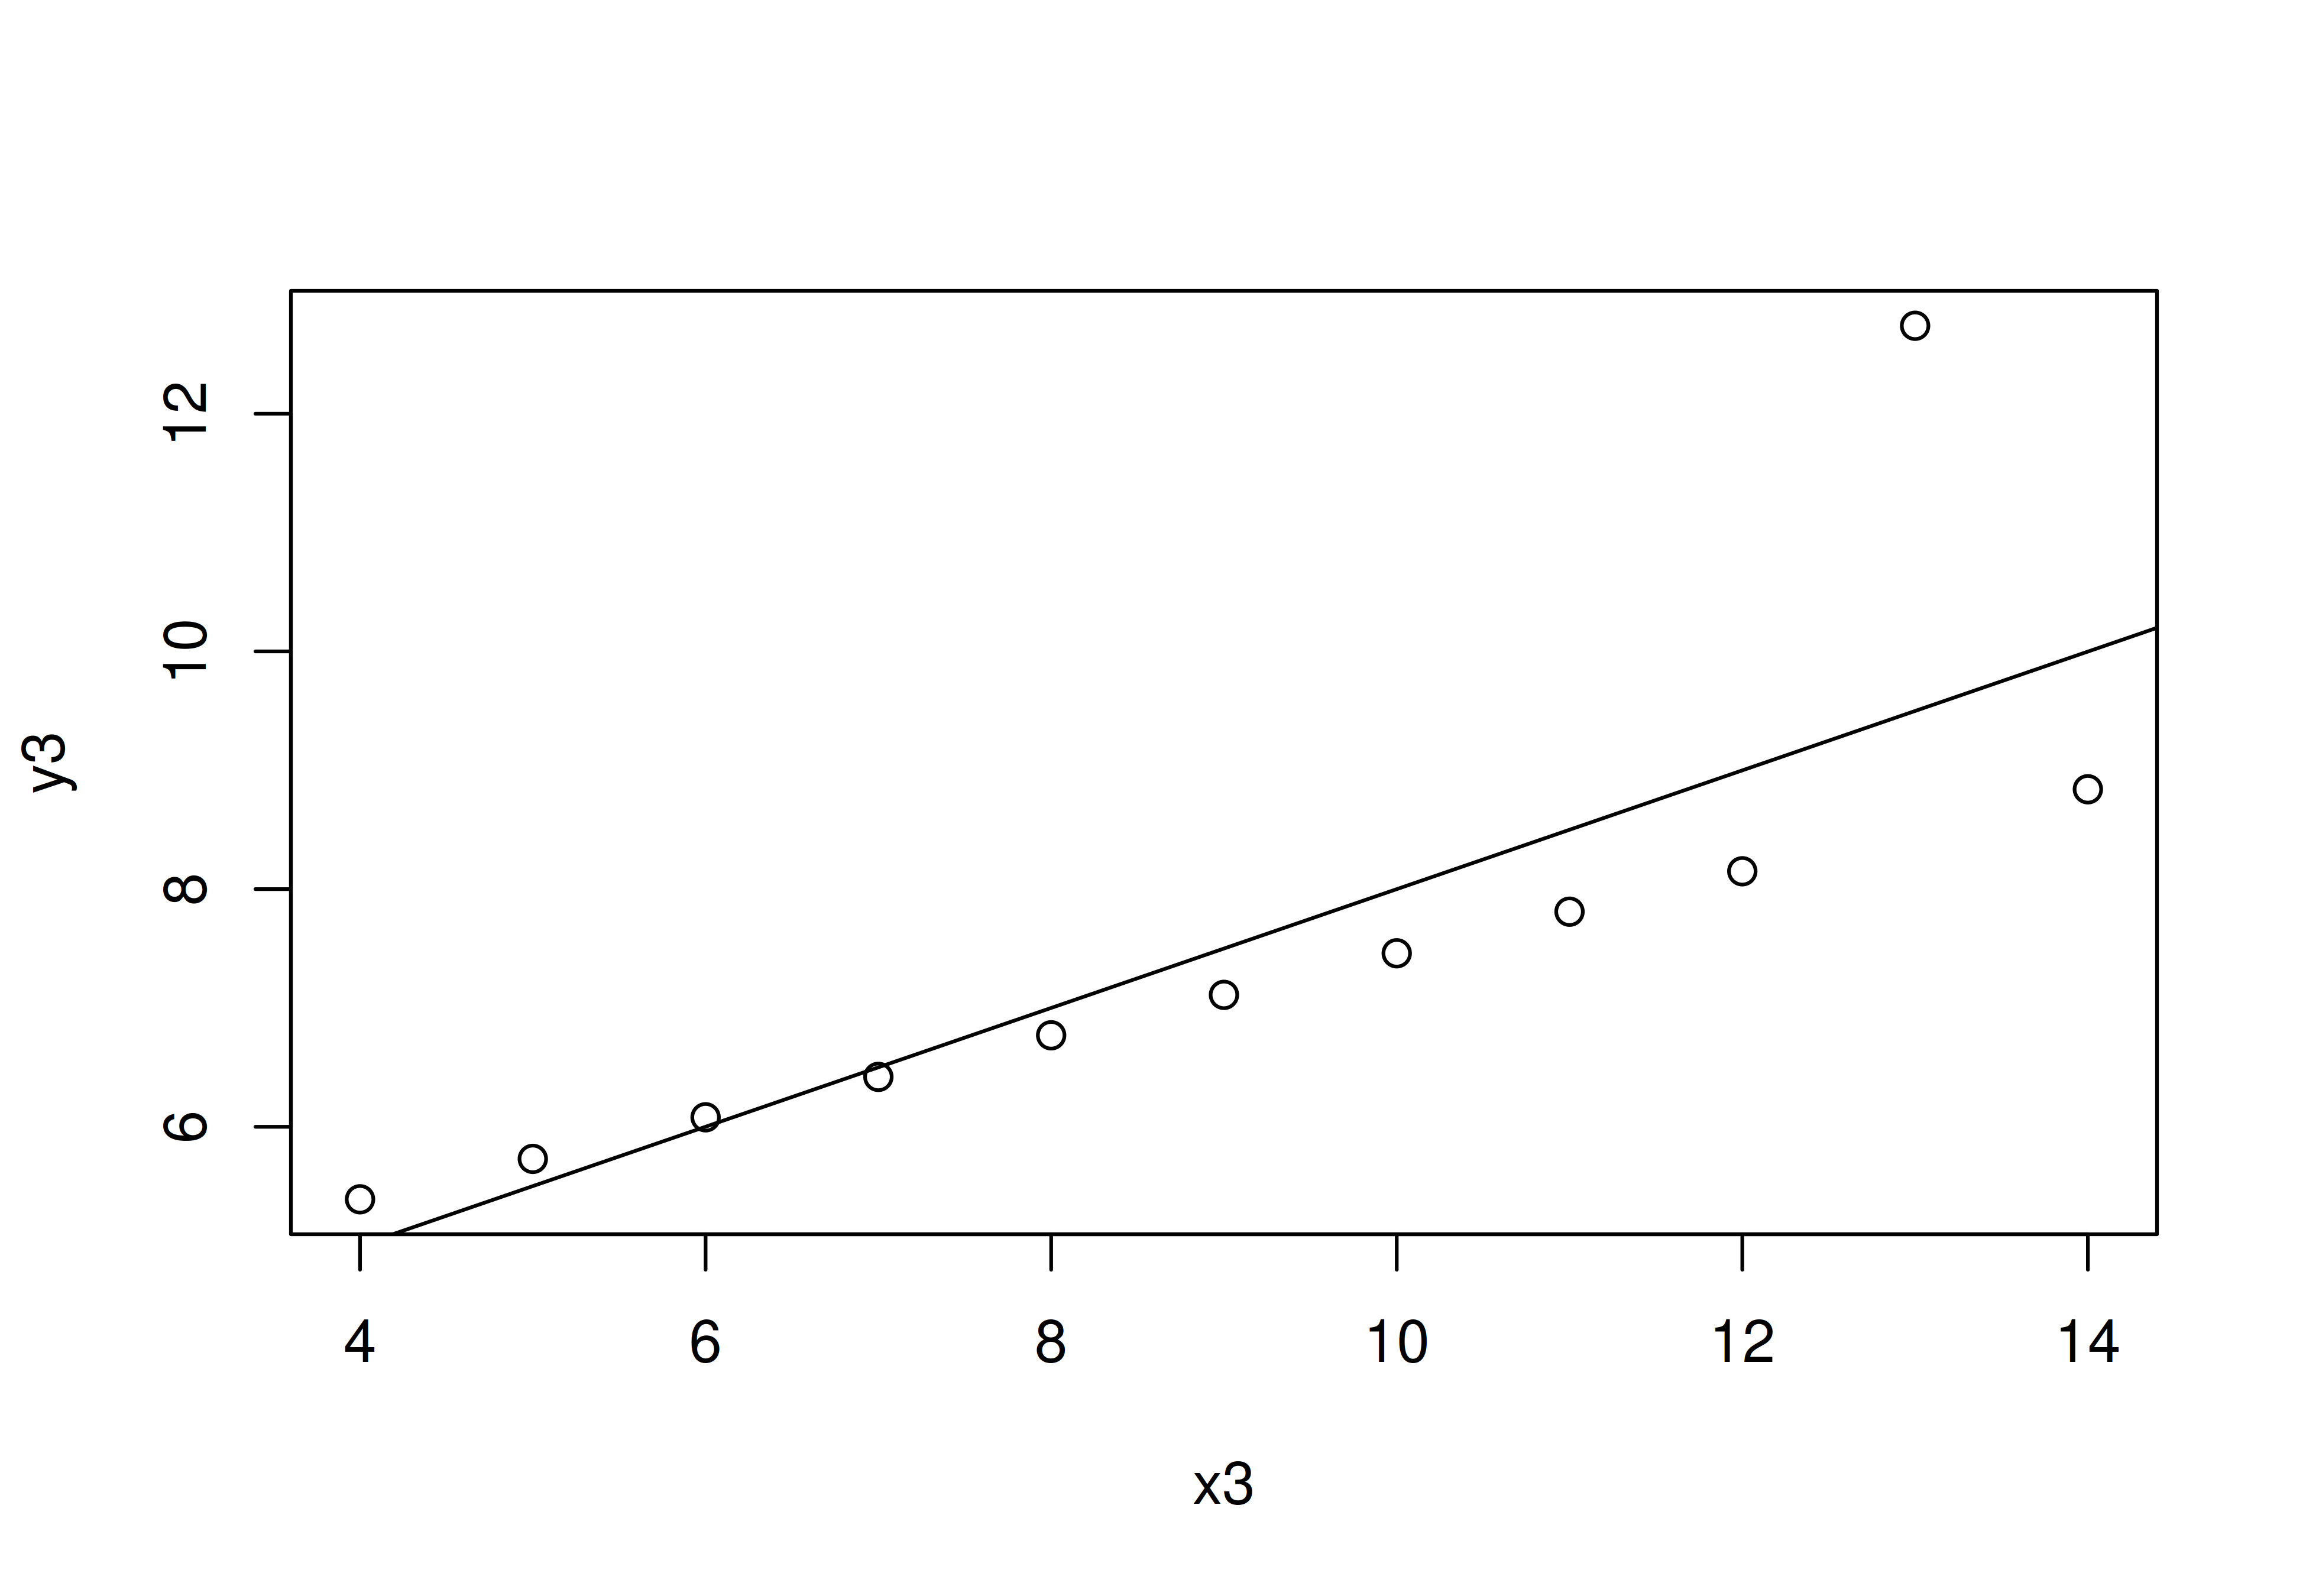
\includegraphics[width=0.49\linewidth]{images/anscombe-3} 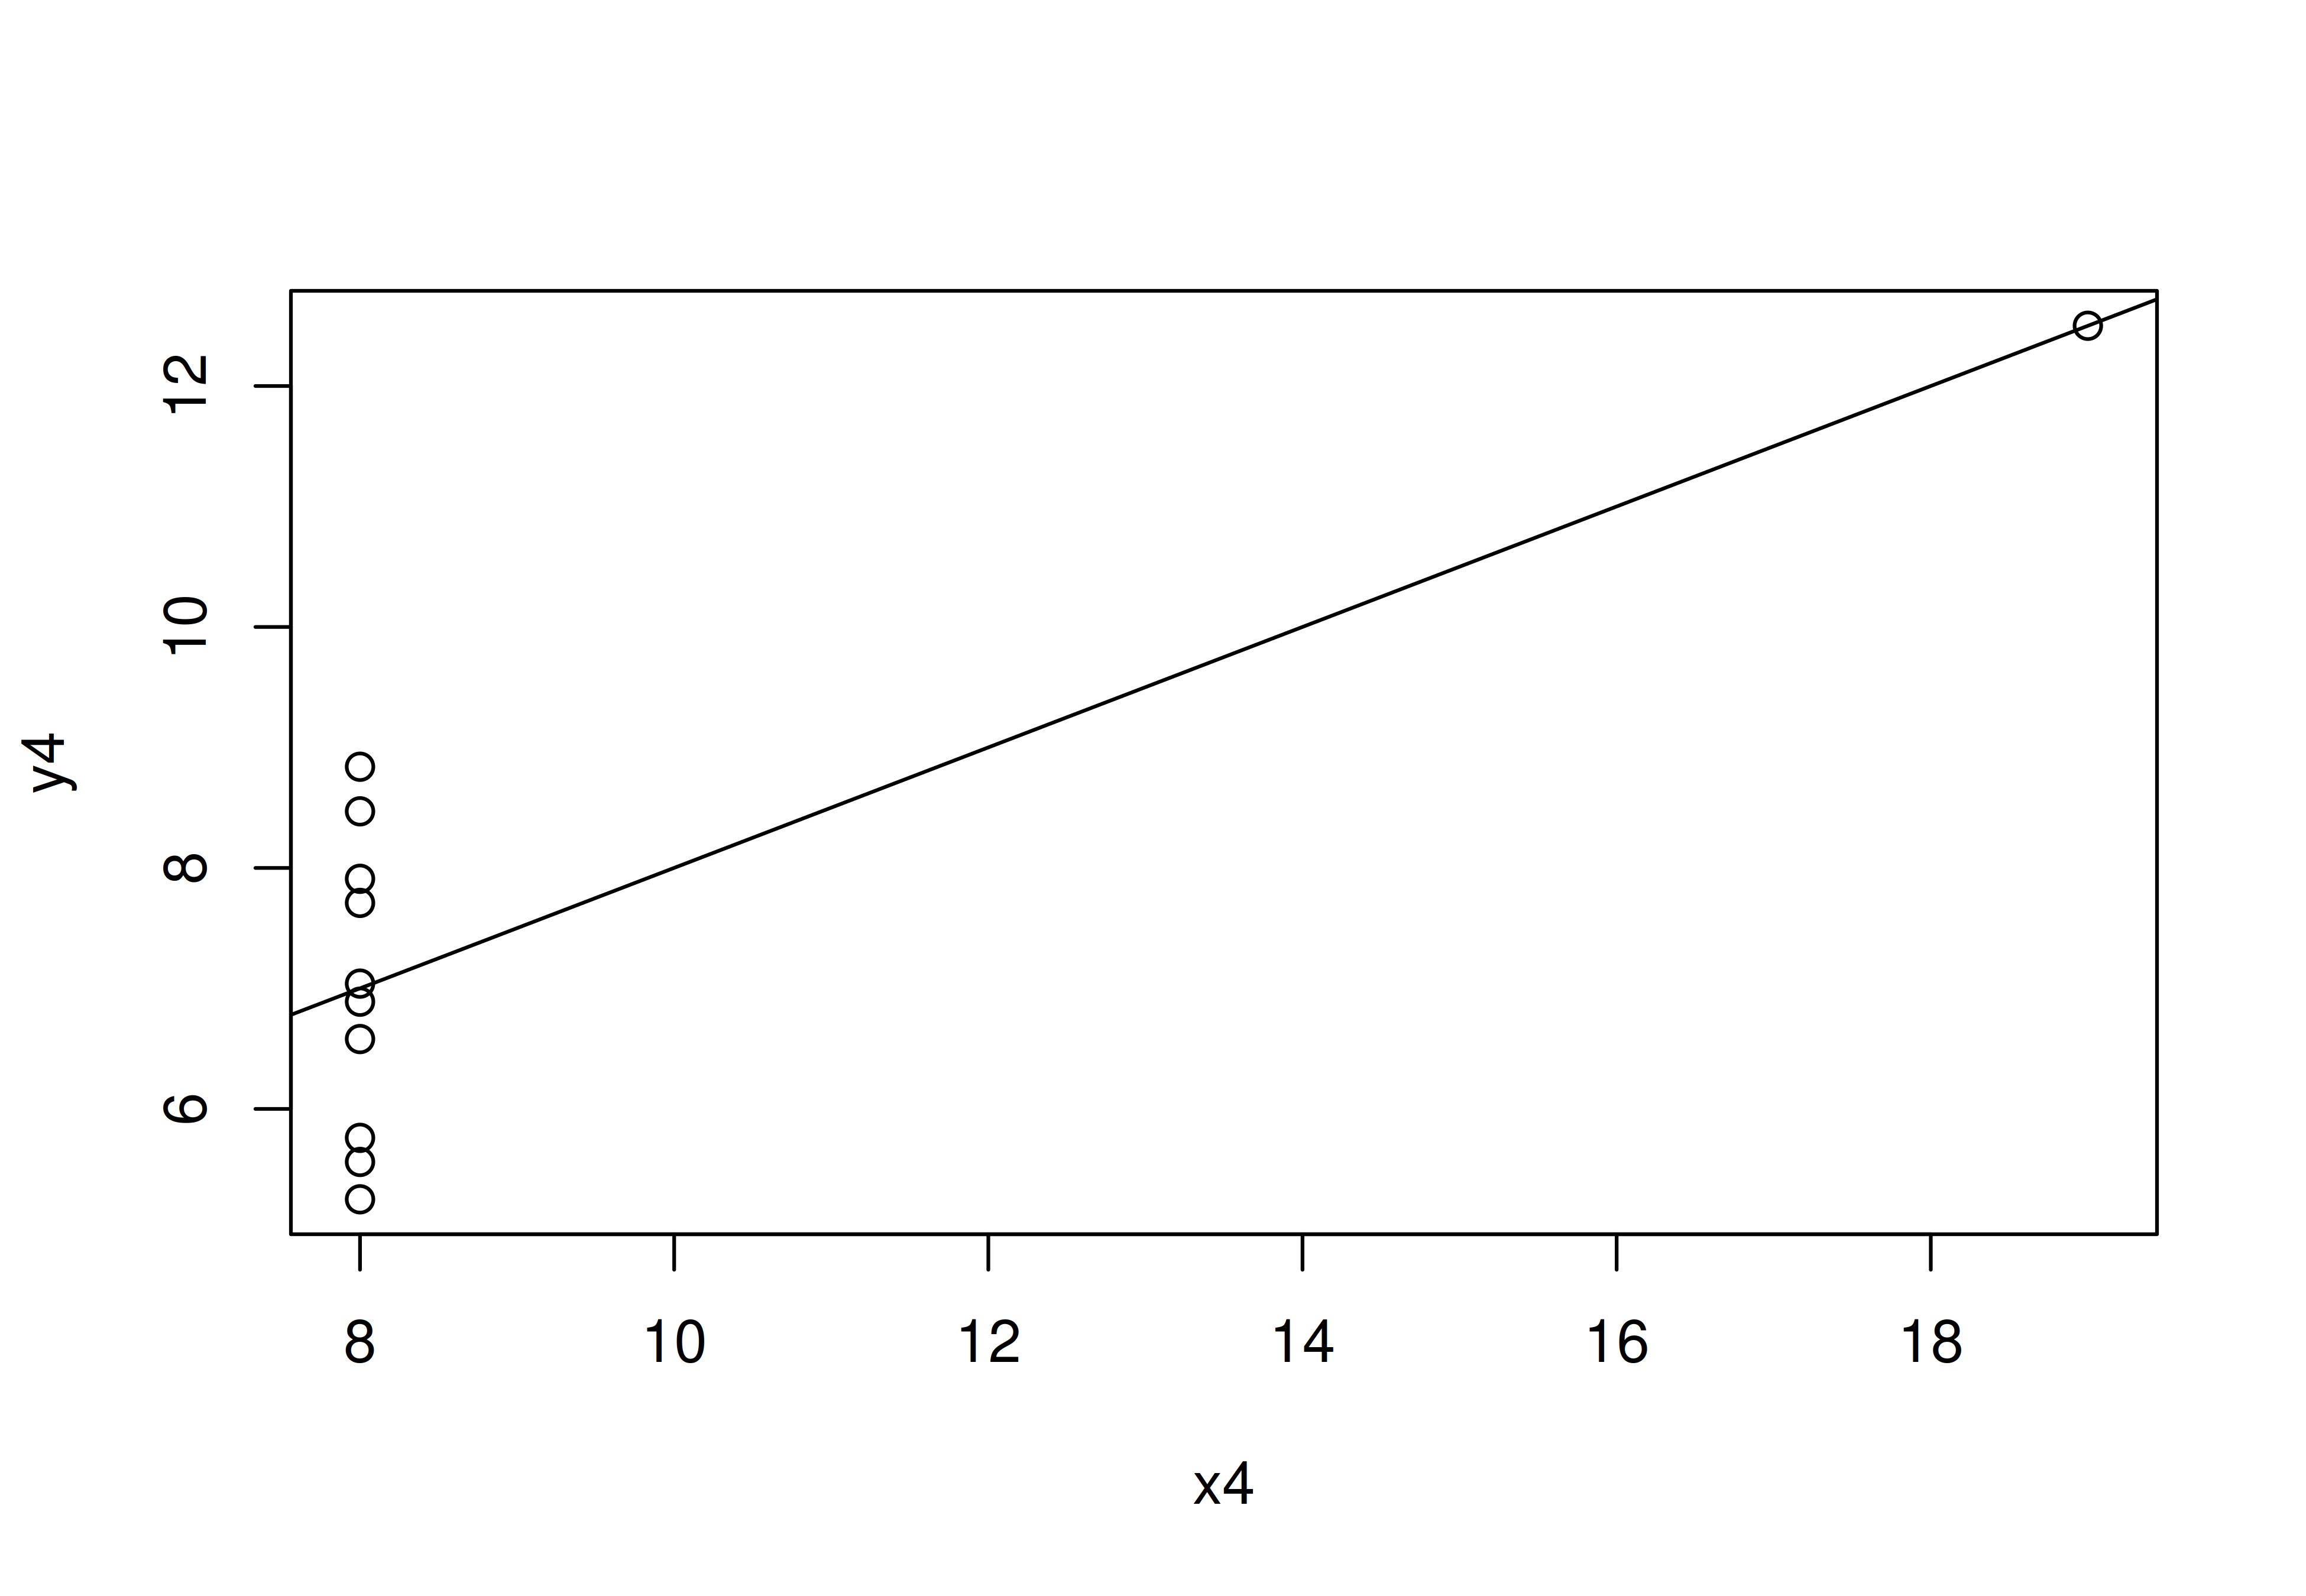
\includegraphics[width=0.49\linewidth]{images/anscombe-4} 

}

\caption{O quarteto de Anscombe.}\label{fig:anscombe}
\end{figure}
\bcenter

Fonte: do Autor.
\ecenter

Ou utilizando o pacote \pkg{ggplot2} \autocite*{R-ggplot2}, obtendo-se a figura \ref{fig:anscombe2}.
\begin{Shaded}
\begin{Highlighting}[]
\FunctionTok{library}\NormalTok{(ggplot2)}
\NormalTok{p1 }\OtherTok{\textless{}{-}} \FunctionTok{ggplot}\NormalTok{(anscombe, }\FunctionTok{aes}\NormalTok{(}\AttributeTok{x =}\NormalTok{ x1, }\AttributeTok{y =}\NormalTok{ y1)) }\SpecialCharTok{+}
  \FunctionTok{geom\_point}\NormalTok{(}\AttributeTok{color =} \StringTok{"darkorange"}\NormalTok{, }\AttributeTok{size =} \FloatTok{1.5}\NormalTok{) }\SpecialCharTok{+}
  \FunctionTok{scale\_x\_continuous}\NormalTok{(}\AttributeTok{breaks =} \FunctionTok{seq}\NormalTok{(}\DecValTok{0}\NormalTok{,}\DecValTok{20}\NormalTok{,}\DecValTok{2}\NormalTok{)) }\SpecialCharTok{+}
  \FunctionTok{scale\_y\_continuous}\NormalTok{(}\AttributeTok{breaks =} \FunctionTok{seq}\NormalTok{(}\DecValTok{0}\NormalTok{,}\DecValTok{12}\NormalTok{,}\DecValTok{2}\NormalTok{)) }\SpecialCharTok{+}
  \FunctionTok{expand\_limits}\NormalTok{(}\AttributeTok{x =} \DecValTok{0}\NormalTok{, }\AttributeTok{y =} \DecValTok{0}\NormalTok{) }\SpecialCharTok{+}
  \FunctionTok{labs}\NormalTok{(}\AttributeTok{x =} \StringTok{"x1"}\NormalTok{, }\AttributeTok{y =} \StringTok{"y1"}\NormalTok{,}
       \AttributeTok{title =} \StringTok{"Dataset 1"}\NormalTok{ ) }\SpecialCharTok{+}
  \FunctionTok{geom\_smooth}\NormalTok{(}\AttributeTok{method =} \StringTok{"lm"}\NormalTok{, }\AttributeTok{se =} \ConstantTok{FALSE}\NormalTok{)}

\NormalTok{p2 }\OtherTok{\textless{}{-}} \FunctionTok{ggplot}\NormalTok{(anscombe, }\FunctionTok{aes}\NormalTok{(}\AttributeTok{x =}\NormalTok{ x2, }\AttributeTok{y =}\NormalTok{ y2)) }\SpecialCharTok{+}
  \FunctionTok{geom\_point}\NormalTok{(}\AttributeTok{color =} \StringTok{"darkorange"}\NormalTok{, }\AttributeTok{size =} \FloatTok{1.5}\NormalTok{) }\SpecialCharTok{+}
  \FunctionTok{scale\_x\_continuous}\NormalTok{(}\AttributeTok{breaks =} \FunctionTok{seq}\NormalTok{(}\DecValTok{0}\NormalTok{,}\DecValTok{20}\NormalTok{,}\DecValTok{2}\NormalTok{)) }\SpecialCharTok{+}
  \FunctionTok{scale\_y\_continuous}\NormalTok{(}\AttributeTok{breaks =} \FunctionTok{seq}\NormalTok{(}\DecValTok{0}\NormalTok{,}\DecValTok{12}\NormalTok{,}\DecValTok{2}\NormalTok{)) }\SpecialCharTok{+}
  \FunctionTok{expand\_limits}\NormalTok{(}\AttributeTok{x =} \DecValTok{0}\NormalTok{, }\AttributeTok{y =} \DecValTok{0}\NormalTok{) }\SpecialCharTok{+}
  \FunctionTok{labs}\NormalTok{(}\AttributeTok{x =} \StringTok{"x2"}\NormalTok{, }\AttributeTok{y =} \StringTok{"y2"}\NormalTok{,}
       \AttributeTok{title =} \StringTok{"Dataset 2"}\NormalTok{ ) }\SpecialCharTok{+}
  \FunctionTok{geom\_smooth}\NormalTok{(}\AttributeTok{method =} \StringTok{"lm"}\NormalTok{, }\AttributeTok{se =} \ConstantTok{FALSE}\NormalTok{)}

\NormalTok{p3 }\OtherTok{\textless{}{-}} \FunctionTok{ggplot}\NormalTok{(anscombe, }\FunctionTok{aes}\NormalTok{(}\AttributeTok{x =}\NormalTok{ x3, }\AttributeTok{y =}\NormalTok{ y3)) }\SpecialCharTok{+}
  \FunctionTok{geom\_point}\NormalTok{(}\AttributeTok{color =} \StringTok{"darkorange"}\NormalTok{, }\AttributeTok{size =} \FloatTok{1.5}\NormalTok{) }\SpecialCharTok{+}
  \FunctionTok{scale\_x\_continuous}\NormalTok{(}\AttributeTok{breaks =} \FunctionTok{seq}\NormalTok{(}\DecValTok{0}\NormalTok{,}\DecValTok{20}\NormalTok{,}\DecValTok{2}\NormalTok{)) }\SpecialCharTok{+}
  \FunctionTok{scale\_y\_continuous}\NormalTok{(}\AttributeTok{breaks =} \FunctionTok{seq}\NormalTok{(}\DecValTok{0}\NormalTok{,}\DecValTok{12}\NormalTok{,}\DecValTok{2}\NormalTok{)) }\SpecialCharTok{+}
  \FunctionTok{expand\_limits}\NormalTok{(}\AttributeTok{x =} \DecValTok{0}\NormalTok{, }\AttributeTok{y =} \DecValTok{0}\NormalTok{) }\SpecialCharTok{+}
  \FunctionTok{labs}\NormalTok{(}\AttributeTok{x =} \StringTok{"x3"}\NormalTok{, }\AttributeTok{y =} \StringTok{"y3"}\NormalTok{,}
       \AttributeTok{title =} \StringTok{"Dataset 3"}\NormalTok{ ) }\SpecialCharTok{+}
  \FunctionTok{geom\_smooth}\NormalTok{(}\AttributeTok{method =} \StringTok{"lm"}\NormalTok{, }\AttributeTok{se =} \ConstantTok{FALSE}\NormalTok{)}

\NormalTok{p4 }\OtherTok{\textless{}{-}} \FunctionTok{ggplot}\NormalTok{(anscombe, }\FunctionTok{aes}\NormalTok{(}\AttributeTok{x =}\NormalTok{ x4, }\AttributeTok{y =}\NormalTok{ y4)) }\SpecialCharTok{+}
  \FunctionTok{geom\_point}\NormalTok{(}\AttributeTok{color =} \StringTok{"darkorange"}\NormalTok{, }\AttributeTok{size =} \FloatTok{1.5}\NormalTok{) }\SpecialCharTok{+}
  \FunctionTok{scale\_x\_continuous}\NormalTok{(}\AttributeTok{breaks =} \FunctionTok{seq}\NormalTok{(}\DecValTok{0}\NormalTok{,}\DecValTok{20}\NormalTok{,}\DecValTok{2}\NormalTok{)) }\SpecialCharTok{+}
  \FunctionTok{scale\_y\_continuous}\NormalTok{(}\AttributeTok{breaks =} \FunctionTok{seq}\NormalTok{(}\DecValTok{0}\NormalTok{,}\DecValTok{12}\NormalTok{,}\DecValTok{2}\NormalTok{)) }\SpecialCharTok{+}
  \FunctionTok{expand\_limits}\NormalTok{(}\AttributeTok{x =} \DecValTok{0}\NormalTok{, }\AttributeTok{y =} \DecValTok{0}\NormalTok{) }\SpecialCharTok{+}
  \FunctionTok{labs}\NormalTok{(}\AttributeTok{x =} \StringTok{"x4"}\NormalTok{, }\AttributeTok{y =} \StringTok{"y4"}\NormalTok{,}
       \AttributeTok{title =} \StringTok{"Dataset 4"}\NormalTok{ ) }\SpecialCharTok{+}
  \FunctionTok{geom\_smooth}\NormalTok{(}\AttributeTok{method =} \StringTok{"lm"}\NormalTok{, }\AttributeTok{se =} \ConstantTok{FALSE}\NormalTok{)}
\end{Highlighting}
\end{Shaded}
\begin{figure}[H]

{\centering 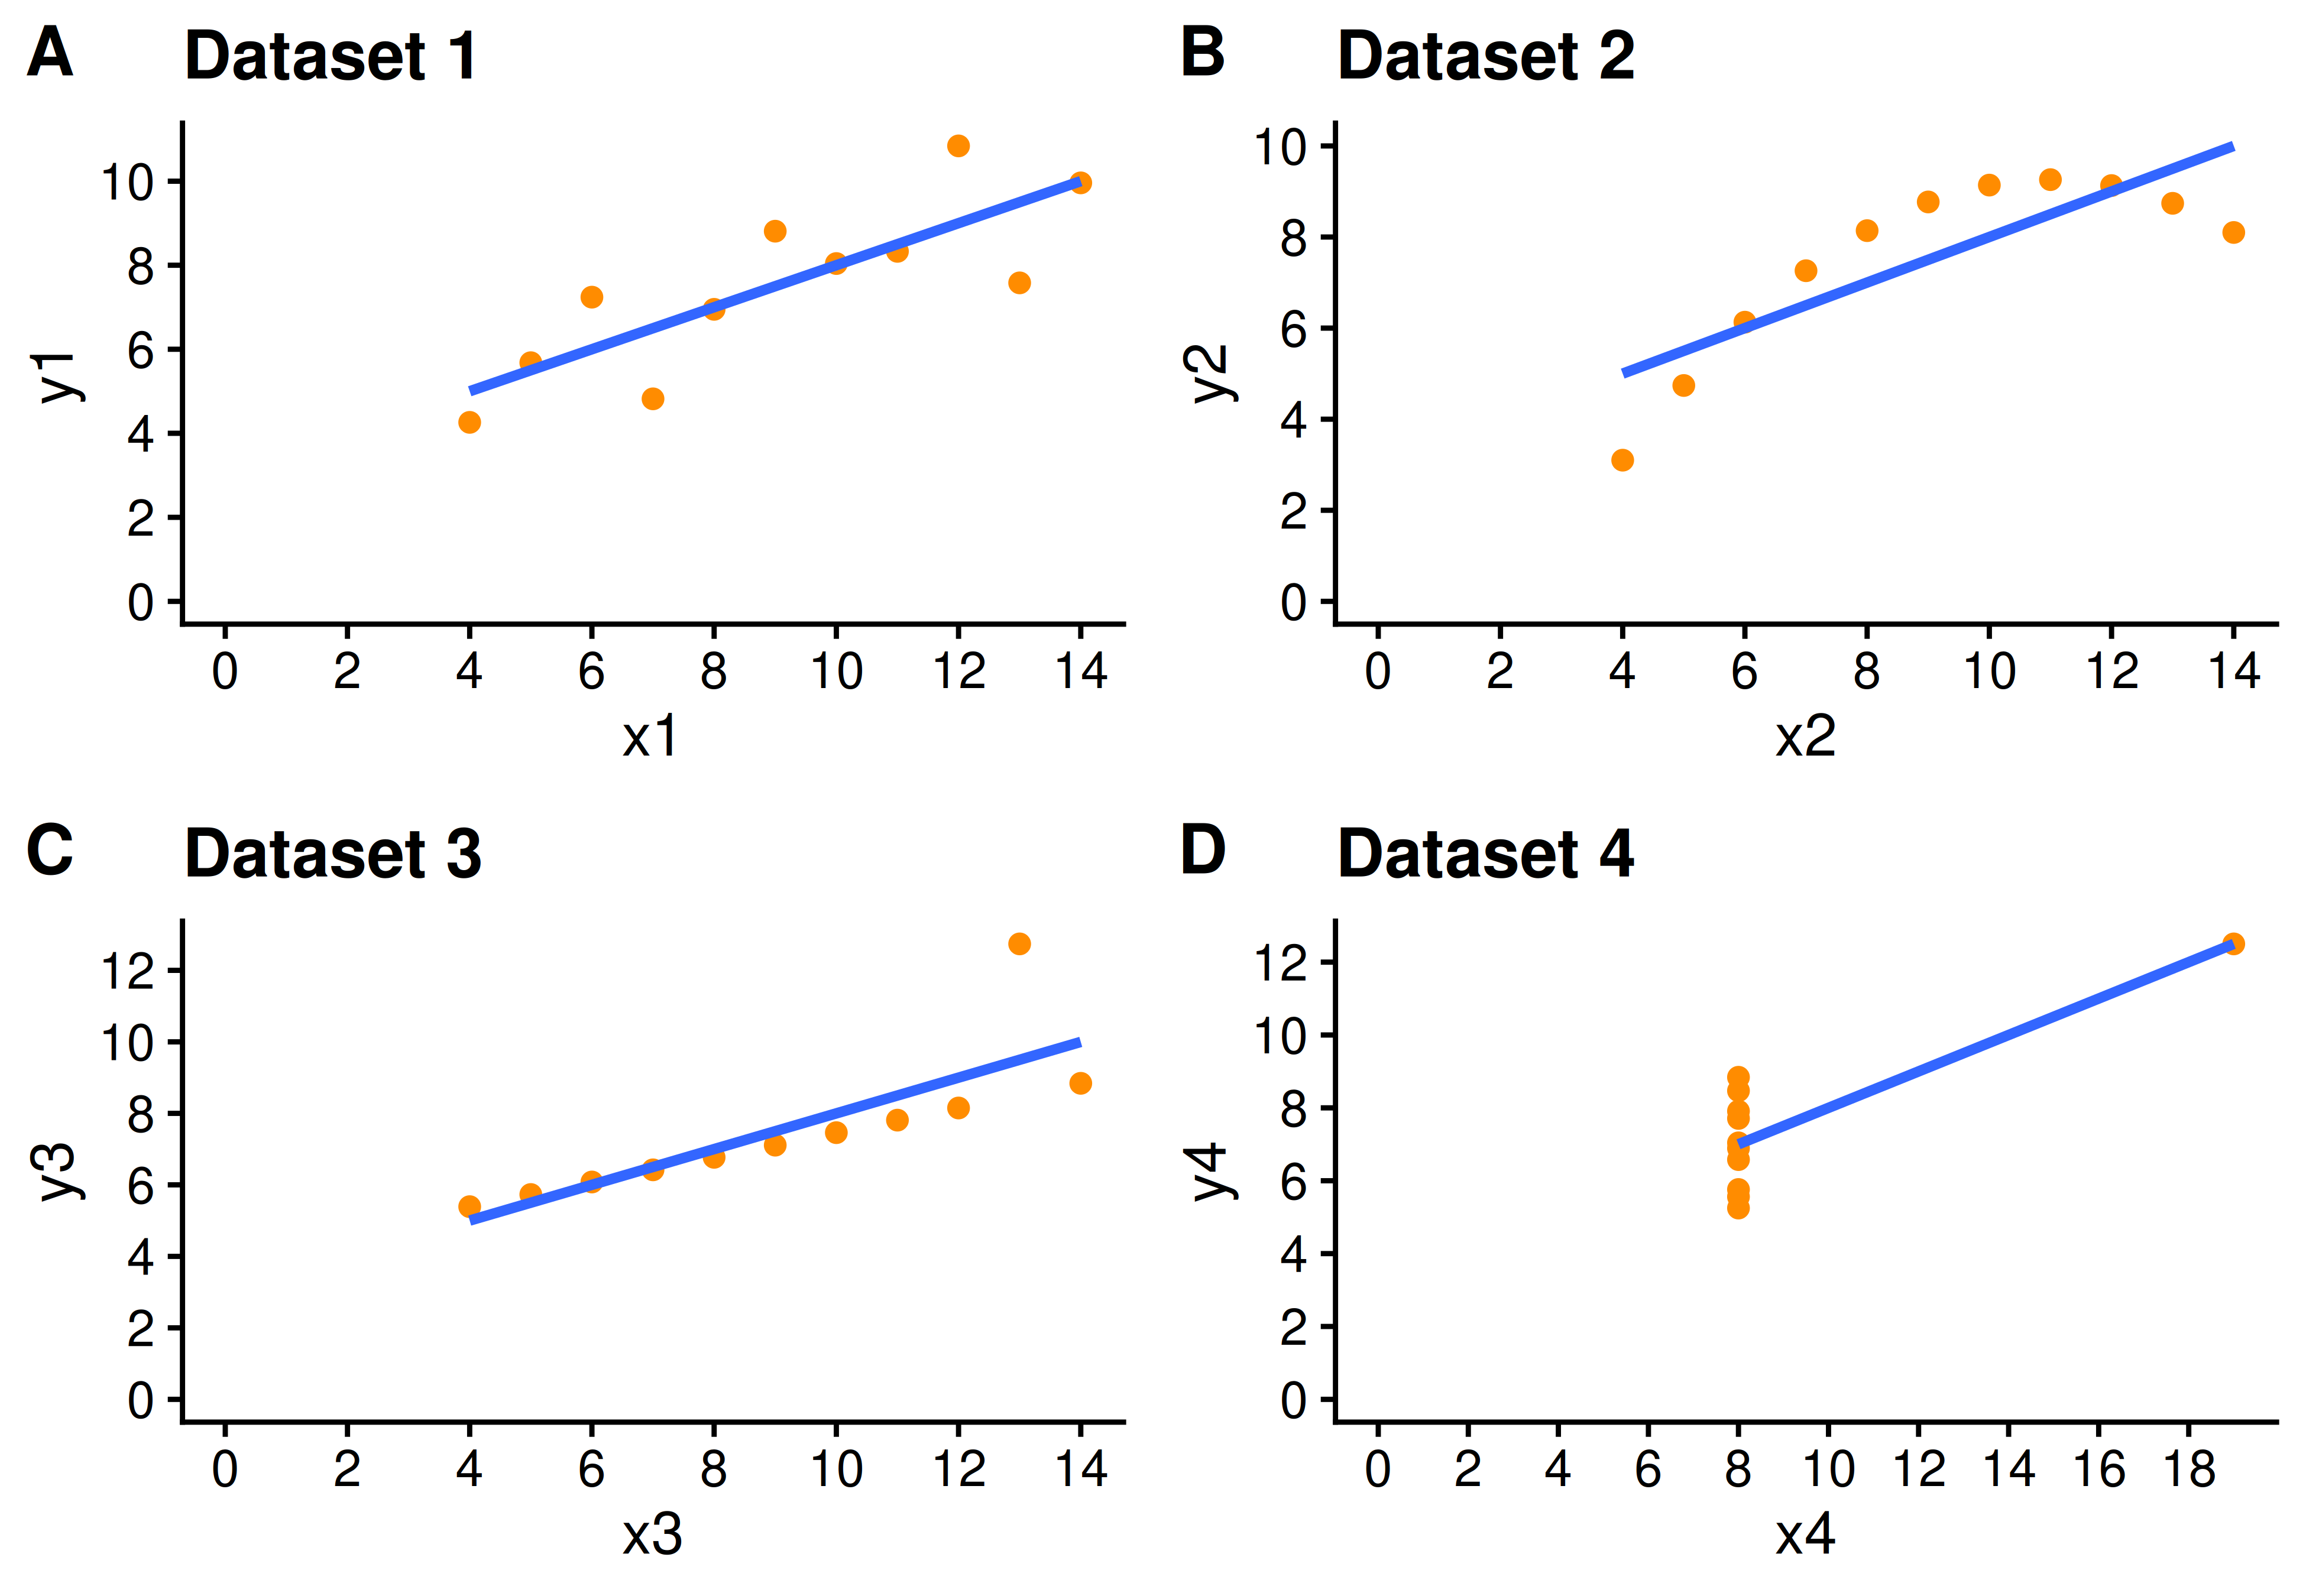
\includegraphics[width=1\linewidth]{images/anscombe2-1} 

}

\caption{O Quarteto de Anscombe}\label{fig:anscombe2}
\end{figure}
\bcenter

Fonte: do Autor.
\ecenter

\chapter*{Capítulo 3}\label{cap3}
\addcontentsline{toc}{chapter}{Capítulo 3}

blablabla

\chapter{Discussão}\label{disc}

blablabla

\chapter{Conclusão}\label{conclusuxe3o}

As conclusões devem responder às questões da pesquisa, em relação aos objetivos
e às hipóteses. Devem ser breves, podendo apresentar recomendações e sugestões
para trabalhos futuros.

\postextual

\begingroup

\printbibliography[title=REFERÊNCIAS]

\endgroup

\markboth{Referências}{REFERÊNCIAS}

\bapendices

\chapter{DESCRIÇÃO 1}\label{appendix-a}

Textos elaborados pelo autor, a fim de completar a sua argumentação. Deve ser
precedido da palavra APÊNDICE, identificada por letras maiúsculas consecutivas,
travessão e pelo respectivo título. Utilizam-se letras maiúsculas dobradas quando
esgotadas as letras do alfabeto.

\textbf{No arquivo Rmd principal}
\begin{Shaded}
\begin{Highlighting}[]
\NormalTok{knitr}\SpecialCharTok{::}\NormalTok{opts\_chunk}\SpecialCharTok{$}\FunctionTok{set}\NormalTok{(}\AttributeTok{echo =} \ConstantTok{FALSE}\NormalTok{, }\AttributeTok{cache =} \ConstantTok{FALSE}\NormalTok{, }\AttributeTok{message=}\ConstantTok{FALSE}\NormalTok{, }
                      \AttributeTok{warning =} \ConstantTok{FALSE}\NormalTok{, }\AttributeTok{fig.ext=}\StringTok{\textquotesingle{}png\textquotesingle{}}\NormalTok{, }\AttributeTok{fig.align=}\StringTok{\textquotesingle{}center\textquotesingle{}}\NormalTok{, }
                      \AttributeTok{fig.path =} \StringTok{"images/"}\NormalTok{, }\AttributeTok{fig.pos =} \StringTok{"H"}\NormalTok{, }\AttributeTok{dev =} \StringTok{"png"}\NormalTok{, }
                      \AttributeTok{dpi =} \DecValTok{600}\NormalTok{, }\AttributeTok{out.width =} \StringTok{"70\%"}\NormalTok{)}
\NormalTok{type }\OtherTok{\textless{}{-}}\NormalTok{ knitr}\SpecialCharTok{::}\NormalTok{opts\_knit}\SpecialCharTok{$}\FunctionTok{get}\NormalTok{(}\StringTok{"rmarkdown.pandoc.to"}\NormalTok{)}
\CommentTok{\# This chunk ensures that the ufscdown package is}
\CommentTok{\# installed and loaded. This ufscdown package includes}
\CommentTok{\# the template files for the thesis.}
\ControlFlowTok{if}\NormalTok{(}\SpecialCharTok{!}\FunctionTok{require}\NormalTok{(remotes))}
  \FunctionTok{install.packages}\NormalTok{(}\StringTok{"remotes"}\NormalTok{, }\AttributeTok{repos =} \StringTok{"http://cran.rstudio.com"}\NormalTok{)}
\ControlFlowTok{if}\NormalTok{(}\SpecialCharTok{!}\FunctionTok{require}\NormalTok{(ufscdown))}
\NormalTok{  remotes}\SpecialCharTok{::}\FunctionTok{install\_github}\NormalTok{(}\StringTok{"lfpdroubi/ufscdown"}\NormalTok{)}
\FunctionTok{library}\NormalTok{(ufscdown)}
\end{Highlighting}
\end{Shaded}
\textbf{No Capítulo \ref{desenvolvimento}:}

\chapter{FOR FUN}\label{appendix-b}

\eapendices

\banexos

\chapter{DESCRIÇÃO 1}\label{descriuxe7uxe3o-1}

São documentos não elaborados pelo autor que servem como fundamentação (mapas,
leis, estatutos). Deve ser precedido da palavra ANEXO, identificada por letras
maiúsculas consecutivas, travessão e pelo respectivo título. Utilizam-se letras
maiúsculas dobradas quando esgotadas as letras do alfabeto.

\textbf{No arquivo Rmd principal}
\begin{Shaded}
\begin{Highlighting}[]
\NormalTok{knitr}\SpecialCharTok{::}\NormalTok{opts\_chunk}\SpecialCharTok{$}\FunctionTok{set}\NormalTok{(}\AttributeTok{echo =} \ConstantTok{FALSE}\NormalTok{, }\AttributeTok{cache =} \ConstantTok{FALSE}\NormalTok{, }\AttributeTok{message=}\ConstantTok{FALSE}\NormalTok{, }
                      \AttributeTok{warning =} \ConstantTok{FALSE}\NormalTok{, }\AttributeTok{fig.ext=}\StringTok{\textquotesingle{}png\textquotesingle{}}\NormalTok{, }\AttributeTok{fig.align=}\StringTok{\textquotesingle{}center\textquotesingle{}}\NormalTok{, }
                      \AttributeTok{fig.path =} \StringTok{"images/"}\NormalTok{, }\AttributeTok{fig.pos =} \StringTok{"H"}\NormalTok{, }\AttributeTok{dev =} \StringTok{"png"}\NormalTok{, }
                      \AttributeTok{dpi =} \DecValTok{600}\NormalTok{, }\AttributeTok{out.width =} \StringTok{"70\%"}\NormalTok{)}
\NormalTok{type }\OtherTok{\textless{}{-}}\NormalTok{ knitr}\SpecialCharTok{::}\NormalTok{opts\_knit}\SpecialCharTok{$}\FunctionTok{get}\NormalTok{(}\StringTok{"rmarkdown.pandoc.to"}\NormalTok{)}
\CommentTok{\# This chunk ensures that the ufscdown package is}
\CommentTok{\# installed and loaded. This ufscdown package includes}
\CommentTok{\# the template files for the thesis.}
\ControlFlowTok{if}\NormalTok{(}\SpecialCharTok{!}\FunctionTok{require}\NormalTok{(remotes))}
  \FunctionTok{install.packages}\NormalTok{(}\StringTok{"remotes"}\NormalTok{, }\AttributeTok{repos =} \StringTok{"http://cran.rstudio.com"}\NormalTok{)}
\ControlFlowTok{if}\NormalTok{(}\SpecialCharTok{!}\FunctionTok{require}\NormalTok{(ufscdown))}
\NormalTok{  remotes}\SpecialCharTok{::}\FunctionTok{install\_github}\NormalTok{(}\StringTok{"lfpdroubi/ufscdown"}\NormalTok{)}
\FunctionTok{library}\NormalTok{(ufscdown)}
\end{Highlighting}
\end{Shaded}
\textbf{No Capítulo \ref{ref-labels}:}

\chapter{for Fun}\label{for-fun}

\eanexos

% ----------------------------------------------------------
% Glossário
% ----------------------------------------------------------
%
% Consulte o manual da classe abntex2 para orientações sobre o glossário.
%
%\glossary

%---------------------------------------------------------------------
% INDICE REMISSIVO
%---------------------------------------------------------------------
%\phantompart
%\printindex
%---------------------------------------------------------------------

\end{document}
